\subsection{Session 2, Exercise 01}

\lineparagraph{Exercise}

Let $\Sigma=\{0,1\}$. Give a deterministic finite automaton that accepts the words that contain an even number of zeros and an odd number of ones.

\lineparagraph{Solution}

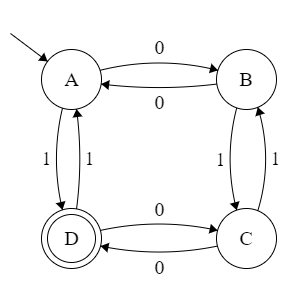
\includegraphics[width=0.4\linewidth]{02/2_1.png}

Proof:

Let's look at what the states mean:

\begin{itemize}
    \item A: State $A$ represents words that contain an even number of $0$'s and $1$'s.
    \item B: State $B$ represents words that contain an odd number of $0$'s and an even number of $1$'s.
    \item C: State $C$ represents words that contain an odd number of $0$'s and an odd number of $1$'s.
    \item D: State $D$ represents words that contain an even number of $0$'s and an odd number of $1$'s.
\end{itemize}

Let's look at the starting state and the accepting and rejecting states:

\begin{itemize}
    \item The starting state is the state that should represent the empty string. The empty string contains zero $0$'s and zero $1$'s, and zero is even, which is represented by $A$, so the starting state is $A$.
    \item The only accepting state is $D$, since we want to accept words that contain an even number of zeros and an odd number of ones, which are represented by $D$.
    \item $A$,$B$ and $C$ are rejecting states, since they represent words that are not in the desired language.
\end{itemize}

Let's look at the transitions:

\begin{itemize}
    \item Transitions triggered by a $0$ input are $A\rightarrow{}B$, $B\rightarrow{}A$, $C\rightarrow{}D$, $D\rightarrow{}C$. In these cases the parity of the $1$'s doesn't change, while the parity of the $0$'s is inverted. If we look back on what the states represent we can verify in all $4$ cases that this is the case.
    \item Transitions triggered by a $1$ input are $A\rightarrow{}D$, $D\rightarrow{}A$, $B\rightarrow{}C$, $C\rightarrow{}D$. In these cases the parity of the $0$'s doesn't change, while the parity of the $1$'s is inverted. If we look back on what the states represent we can verify in all $4$ cases that this is the case.
\end{itemize}